Die Rasterisierungspileline und deren Hardwarebeschleunigung war das bisherige sehr effiziente \glqq state-of-the-art\grqq{} Bilderzeugungsverfahren. Mit der hardwareunterstützten 
Strahlenverfolgung scheint es sich nun zu aktuell zu verschieben \cite{Barre-Brisebois2019}. 
Zu Beginn der Rasterisierung haben wir die Eckpunkte der bereits verarbeiteten, transformierten, projizierten Geometrie mit möglichen
Beleuchtungsinformationen aus den vorherigen Berechnungen vorliegen (weiterführende Literatur zu der modernen
Renderingpipeline \cite{akenine2018real}). 
Mit Hilfe der Rasterisierung wird nun die Farbe jedes einzelnen Pixels bestimmt \cite{RasterisierungImplementierung}. Es ist also die Aufgabe der Rasterisierung herauszufinden, 
welche Geometrie welchen Pixel zu welchen Anteil bedeckt und wie die Shading Informationen zur Farbgebung des Pixels beitragen. 
Aufgrund dieser Vorgehensweise spricht man auch von einem objektbasierten Bilderzeugungsverfahren.

\begin{tcolorbox}
    \begin{algorithm}[H]
        \caption{Rasterisierungsalgorithmus}
        \begin{algorithmic}[1]
        \Procedure{Rasterisierung}{$Dreiecke$}\Comment{Pipelining der Dreiecke}
        \For{dreieck $\in$ Dreiecke}    
            \State projeziereEckpunkteInBild();
            \For{(x,y) $\in$ image}
                \If{(x,y) im projezierten Dreieck enthalten}
                \State färbe Pixel mit dreieck.farbe;
                \EndIf
            \EndFor
        \EndFor
        \EndProcedure
        \end{algorithmic}
        \label{alg:RasterizationAlg}
    \end{algorithm}
\end{tcolorbox}

Die bereits angesprochene Effizienz hat der Rasterisierungsalgorithmus \ref{alg:RasterizationAlg} der rechengünstigen Operation des Projizierens und der 
einfachen Umsetzung eines Pixelzugehörigkeitstests für ein Dreieck zu verdanken. Desweiteren lassen sich verschiedene sehr effiziente Verbesserungen vornehmen, 
z.B. lassen sich Bounding-Boxen verwenden, womit sich die untersuchten Pixel für jedes Dreieck (stark) reduzieren lassen. 

%%%%%%%%%%%%%%%%%%%%%%%%%%%%%%%%%%%%%%%%
%%%%%%%% wie Rasterisierung funktioniert 
%%%%%%%%%%%%%%%%%%%%%%%%%%%%%%%%%%%%%%%%
\begin{figure}[H]
    \begin{tcolorbox}
        \centering
        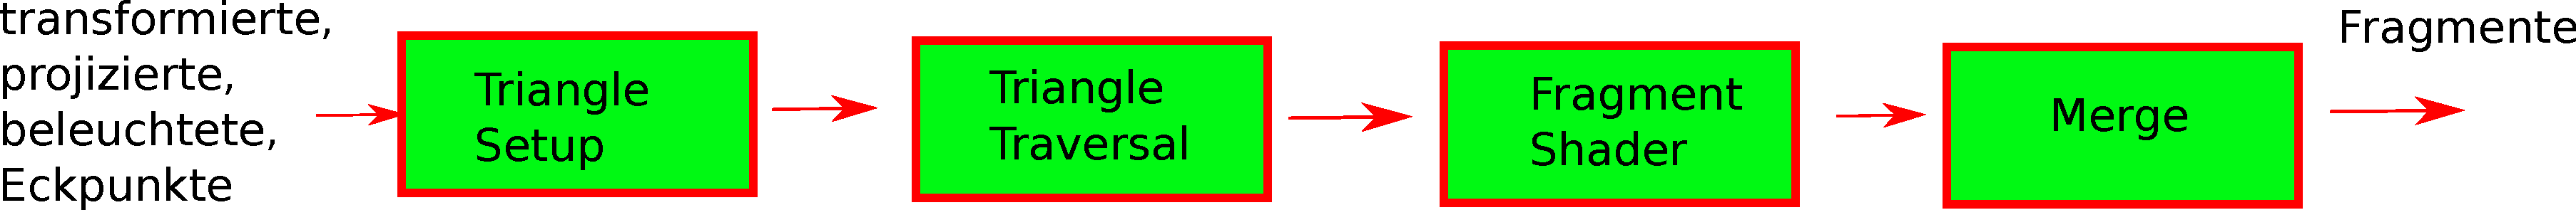
\includegraphics[width=\linewidth]{content/PathTracer/Bilder/Rasterisierung.pdf}
        \end{tcolorbox}
    \caption{Ablauf der Rasterisierung}
    \label{pic:Rasterisierungsablauf}
\end{figure}

\vspace*{3cm}        
Zuallererst befindet man sich im \nameref{pic:Rasterisierungsablauf}(siehe Abbildung \ref{pic:Rasterisierungsablauf}) beim \textit{Triangle Setup}. 
Unbeeinflussbar vom Programmierer werden hier Daten berechnet, welche zur Pixeleinfärbung
benötigt werden. Beim darauffolgenden Schritt, dem \textit{Triangle Traversal}, werden die \textit{Fragmente} erzeugt, indem diejenigen Pixel bestimmt werden, welche innerhalb des Dreiecks liegen. 
Als freiprogrammierbare Shadereinheit können im \textit{Fragment Shader} vom Programmierer weitere Berechnungen vorgenommen werden. Dazu zählt eine pro Pixel Beleuchtungsberechnung (Phong Shading).
Das abschließende nicht komplett freiprogrammierbare, aber hoch konfigurierbare \textit{Merging} hat eine besondere Aufgabe beim Abspeichern der Farbe für
jeden Pixel im color Buffer. Zur Bestimmung der aktuellen Farbe wird nun auch das Problem der Sichtbarkeit von Objekten angegangen. Zu den Depth-Werten, welche wir als Tiefe beim 
Viewport Transform gespeichert haben, gibt es hier Zugang zum Depth-Buffer. Dieser Depth-Buffer speichert anfangs überall den Wert inf. Beim Durchlauf der Geometrie wird nun jeweils für jeden Pixel,
der die Geometrie bedeckt der color und depth buffer wie folgt aktualisiert: Ist der verglichene Tiefenwert des vom Objekt erzeugten Fragment kleiner als der Wert
im Tiefenbuffer für den betroffenen Pixel, so schreibt er diesen Tiefenwert in den Depth-Buffer und auch der color Buffer mit der Fragmentfarbe aktualisiert.
Falls nicht passiert nichts und das nächste Primitiv bzw. Fragment wird betrachtet. 
Eine Möglichkeit ist die Ausgabe, bestehend aus Lichter, Normalen, Tiefenwert, Farbe (sog. \textit{GBuffer}) in mehrere verschiedene \textit{render targets} zu schreiben. 
Wir werden zur Beschleunigung der globalen Beleuchtung durch einen \nameref{ch:Content1:sec:Path Tracer} einen solchen durch Rasterisierung berechneten \textit{GBuffer}(siehe auch
Abschnitt \ref{pic:Render Graph}) verwenden.
\vfill

\subsection{Beschränktheit}
\label{sec:Rasterisierung:Beschränktheit}

\begin{figure}[H]
    \begin{tcolorbox}
    \centering
    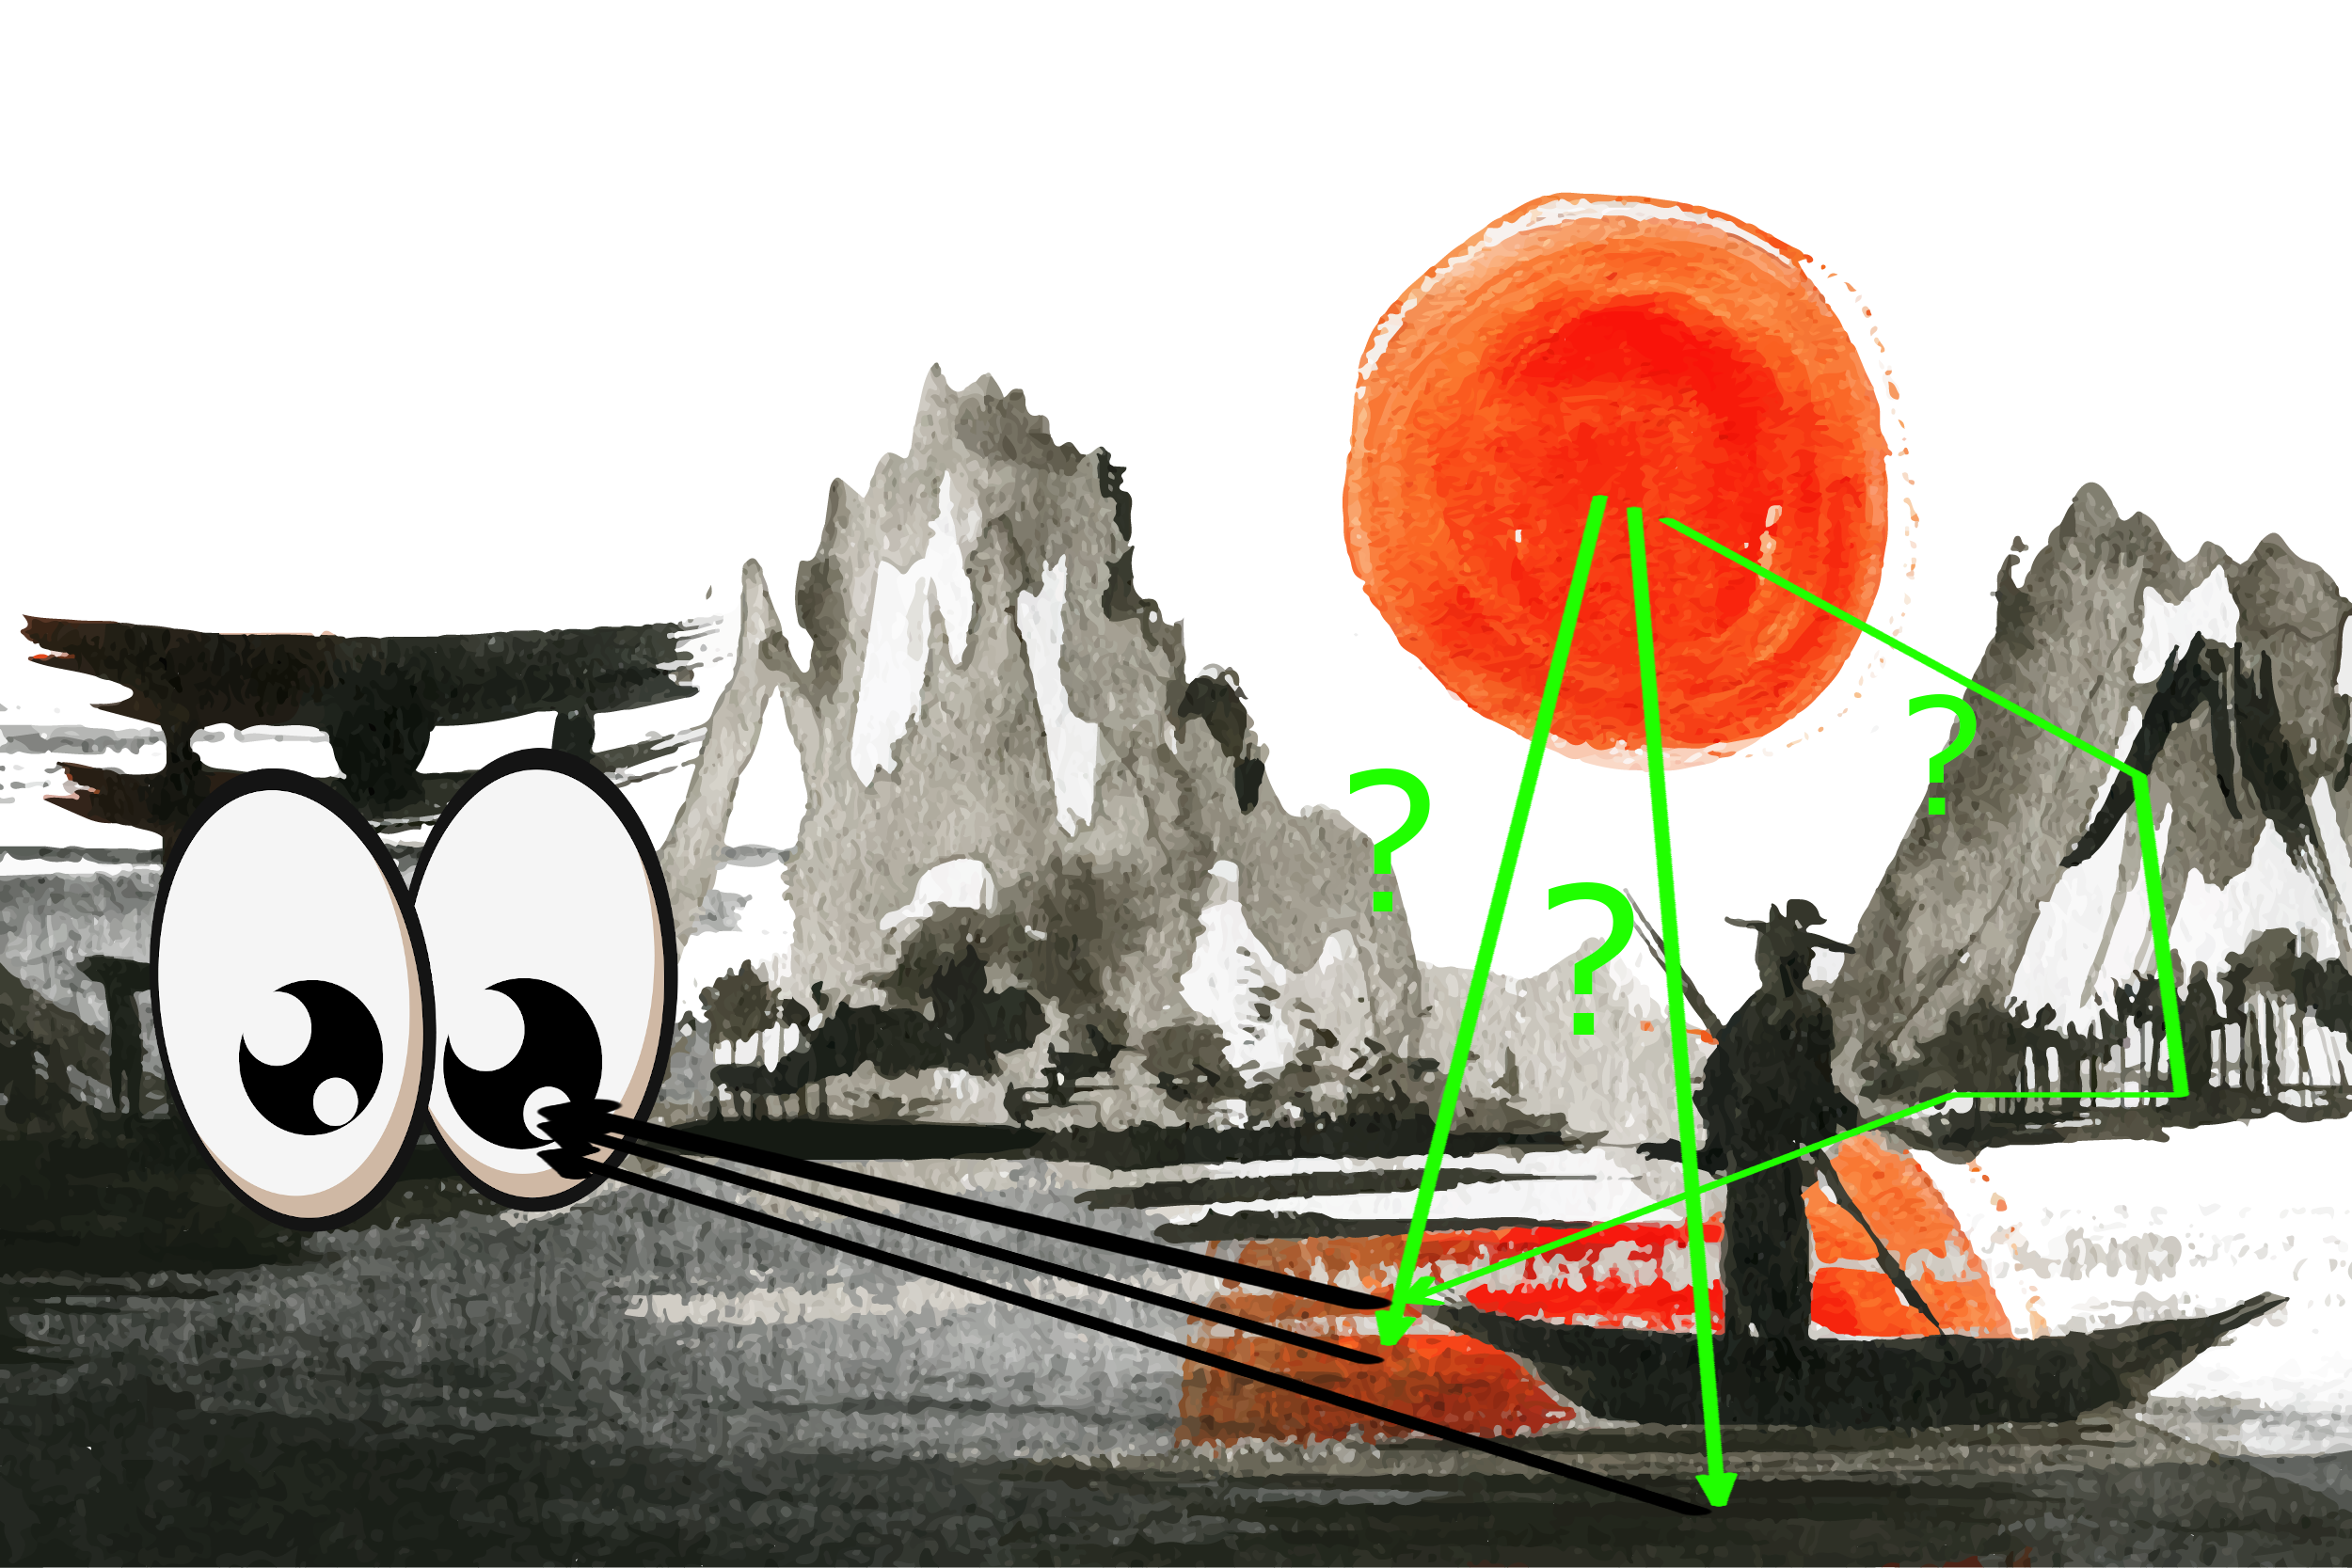
\includegraphics[width=\linewidth]{content/PathTracer/Bilder/RasterizerGuide.png}
    \end{tcolorbox}
    \caption{Ablauf der Rasterisierung}
    \label{pic:RasterizerGuide}
\end{figure}

Ihre bisherige weite Verbreitung hatte die Rasterisierung der Objektorientierung zu verdanken: massives paralleles Arbeiten, Ignorieren von (großen) leeren Bereichen und
Ausnutzen von Cachekohärenzen gehören zu den Eigenschaften, welche die enorme effiziente, schnelle Abarbeitung bzw. (relativ) geringe aufzuwendende Rechenleistung begründen.
Jedoch liegt in ihr auch die Crux.
Die Abbildung der Farbe eines Geometrie/Dreiecks auf einen Pixel simuliert
den physikalischen Lichttransport nicht korrekt! Die physikalische Optik lehrt uns das Verfolgen von weiteren (sekundären) Strahlen 
(siehe grüne Pfeile in Abbildung \ref{pic:RasterizerGuide})abseits des Primärstrahls, der von 
Sichtebene zum Objekt verläuft und durch die Rasterisierung im Gegensatz zu den Sekundärstrahlen abgedeckt wird. Abbildung \ref{pic:RasterizerGuide} verdeutlicht das 
Problem der Objektorientierung und deren Problem mit Sekundärstrahlen. So können Effekte, welche diese Sekundärstrahlen involvieren, 
entweder nicht oder nur (unzureichend befriedigend) dargestellt werden (Spiegelungen, Schatten und Pfade mit größerer Pfadlänge). \par

Die enormen Leistungsanforderungen von Technologien, welche diesen physikalisch korrekten Lichttransport möglich machen, haben sie bisher für Echtzeitanwendungen ausgeschlossen 
und führten zu nicht physikalisch korrekten Approximationstechnicken.
In heutigen modernen Grafikprogrammierschnittstellen (Vulkan, DirectX) jedoch befindet sich Raytracing-Funktionalität, welche auf Hardwareseite unterstützt wird.
Diese Unterstützung erlaubt neuerdings effizientere image-ordered Bilderstellungen in Echtzeit.  
Aktuelle Bemühungen gehen nun daran Strahlenerzeugung und Rasterisierung zu kombinieren. \cite{Barre-Brisebois2019} stellte
mit dem Spiel \textit{PICA PICA} eine solche Rendering-Pipeline vor, welche mithilfe von Path Tracing
(siehe Abschnitt \ref{ch:Content1:sec:Path Tracer}) arbeitet. Dabei wird der G-Buffer
(Texturen die Position, Normalen, Belichtung eines Bildes speichern) noch über Rasterisierung berechnet. Direkten Schatten kann man durch
rechengünstigere Approximationstechnicken oder durch das Verschießen von Strahlen bekommen. Diese Option verspricht eine Anpassungsfähigkeit der Pipeline nach Leistungsfähigkeit der Hardware. Ähnlich können nun
Reflexionen, Global Illumination, Ambient Occlusion und Transmission durch Verschießen von Strahlen oder auf Compute Shader ausgeführt werden (wieder je nach 
Hardwareleistung). Einzig direkte Beleuchtung sowie Post-Processing Effekte laufen nur über Compute-Shader. \par

Wir wollen diesen Ansatz in dieser Arbeit aufnehmen. Berechnung des \textit{GBuffer}'s mit Hilfe von Rasterisierung und globale Beleuchtung durch 
einen \nameref{ch:Content1:sec:Path Tracer} erreichen. Da trotz hardwarebeschleunigtes Strahlenverschießen unsere Anzahl an Strahlen beschränkt ist, 
beschäftigen wir uns innerhalb dieser Arbeit mit einem temporalen Algorithmus (siehe Kapitel \ref{ch:Temporaler Algorithmus}), der die visuelle Qualität nicht 
durch Verschießen von mehr Strahlen, sondern durch eine zeitlich stabile \nameref{ch:Content1:sec:blue noise} Fehlerverteilungen im Bildraum erreicht.